
\section{Evaluation}\label{sec:eval}

We evaluate \name{} along 3 metrics: (1). cost, (2). latency, and (3).
expressiveness, to answer the following questions:

\begin{enumerate}

    \item What is the cost of running applications on \name{} and how does it
    compare to existing serverless workflow systems? Specifically, how much
    additional costs does the \name{} runtime incur in Lambda duration
    billing? And how much does it cost to write and read checkpoints to and
    from the intermediary data store?

    \item What is the latency performance of representative applications on
    \name{}? And how does it compare to existing serverless workflow systems?

    \item How expressive is the \name{} IR? Can one build complex, real-world
    applications with \name{}?

\end{enumerate}


We use a suite of micro- and macro-benchmarks. The micro-benchmarks target the
basic operations of \name{} (e.g., invoking a continuation, checkpointing,
etc.) and building-block orchestration patterns (e.g., chaining, fan-out and
fan-in) to understand \name{}'s performance and cost characteristics.

The macro-benchmarks consists of 4 real-world applications, taken from
serverless repositories and prior research work, and assesses \name{}'s
expressiveness and end-to-end performance and costs.

We show that 

\begin{itemize}

    \item over 97\% of \name{}'s latency overhead comes from API calls to
    Lambda and data stores, which means the bulk of \name{}'s performance will
    automatically improve with the underlying platform (e.g., a faster Lambda
    or data store) without any modification to \name{} itself.

    % \item The additional Lambda duration billing for executing \name{} runtime
    % is negligible across all data sizes

    \item \name{} is slightly faster (11-28\%) in chaining performance and
    much faster in parallel fan-out and fan-in performance (up to 4.58x),
    especially at higher level of parallelism, than Step Functions.

    \item \name{} delivers more than one order-of-magnitude cost savings for
    almost all applications we evaluated, even when using the more expensive
    DynamoDB as the intermediary data store. The applications we use cover all
    orchestration patterns that Step Functions currently support.

    \item \name{} is able to express all orchestration patterns that Step
    Functions currently support. Additionally, with the ExCamera
    implementation, we demonstrate that \name{} can express fold or for loops
    and support pipeline parallelism, neither of which is expressible in Step
    Functions.

\end{itemize}

\subsection{Experimental setup}

We run all experiments on AWS, region \texttt{us-west-1} and costs numbers
reflect \texttt{us-west-1} pricing. We configure lambdas to 128MB memory size
unless otherwise specified and use on-demand capacity mode for DynamoDB. To
avoid function cold starts, we pre-warm functions by running the workflow a
few doze times before collecting measurement.

% S3 buckets all have Versioning turned on.

We compare against Step Functions as the baseline. All applications in the
evaluation are written as Step Functions state machines and \name{} versions
are compiled from the Step Functions definitions, with the only exception of
ExCamera due to limitations of the AWS State Language which we discuss in
Sec.~\ref{sec:}.

% We compare against Step Functions' \emph{Standard} Workflows as the baseline. 


All Step Functions workflows are executed as \emph{Standard}
workflows~\cite{aws-step-functions-standard-vs-express}. Similar to \name{},
the Standard workflows persist execution states on every state transition
(i.e., completing one function and starting the next function), and always
return exactly one response for one workflow
invocation~\cite{aws-step-functions-exec-gntee}.

We do not consider Step Functions' Express Workflows in our comparison because
of its weaker execution guarantee, namely the same invocation could result in
multiple and potentially diverging results if any part of the workflow logic
is nonidempotent~\cite{aws-step-functions-exec-gntee}.

Note that even though Step Functions claims that the Standard Workflows
provides "exactly-once workflow
execution"~\cite{aws-step-functions-exec-gntee}, it is not clear whether it
implies exactly-once execution for component functions of the workflows. Our
interpretation is that the internal states of a standard workflow will appear
to execute exactly once, but component functions might not run exactly-once
due to failures and retries, which is identical to \name{}.

\subsection{Microbenchmarks}

\begin{figure}[t!]
    \centering
    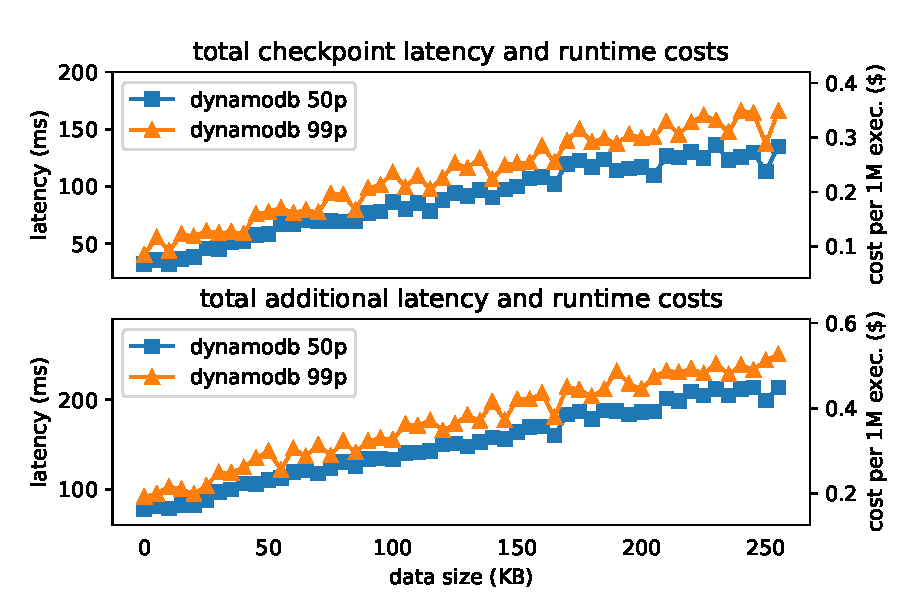
\includegraphics[width=\columnwidth]{figures/TotalAdditionalLatency.pdf}
    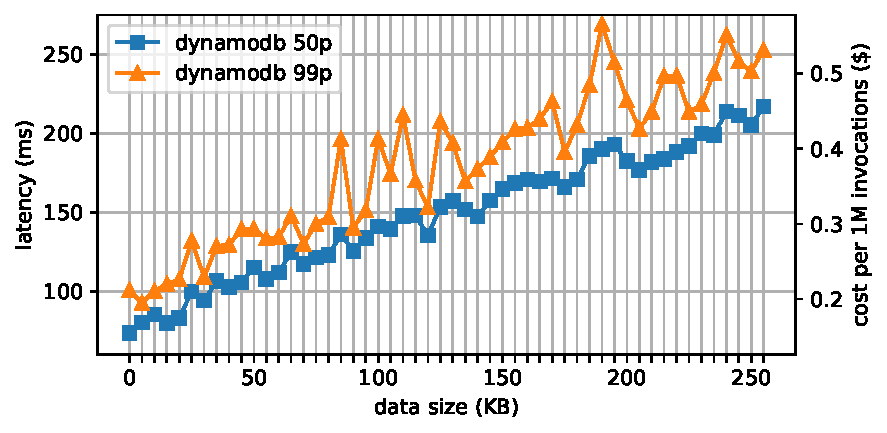
\includegraphics[width=\columnwidth]{figures/TotalAdditionalLatencyNCosts.pdf}
    \caption{Total latency for a state transition}
    % \caption{Total latency for a single state transition. We use a
    % chain of two functions (\texttt{F->G}) that simply return their input.
    % \texttt{data size} is the output data size of \texttt{F}, which in turn is
    % the amount of data \texttt{F} writes to checkpoint and the input data size
    % of \texttt{G}.}
    \label{fig:totallatency}
\end{figure}

\begin{figure}[t!]
    \centering
    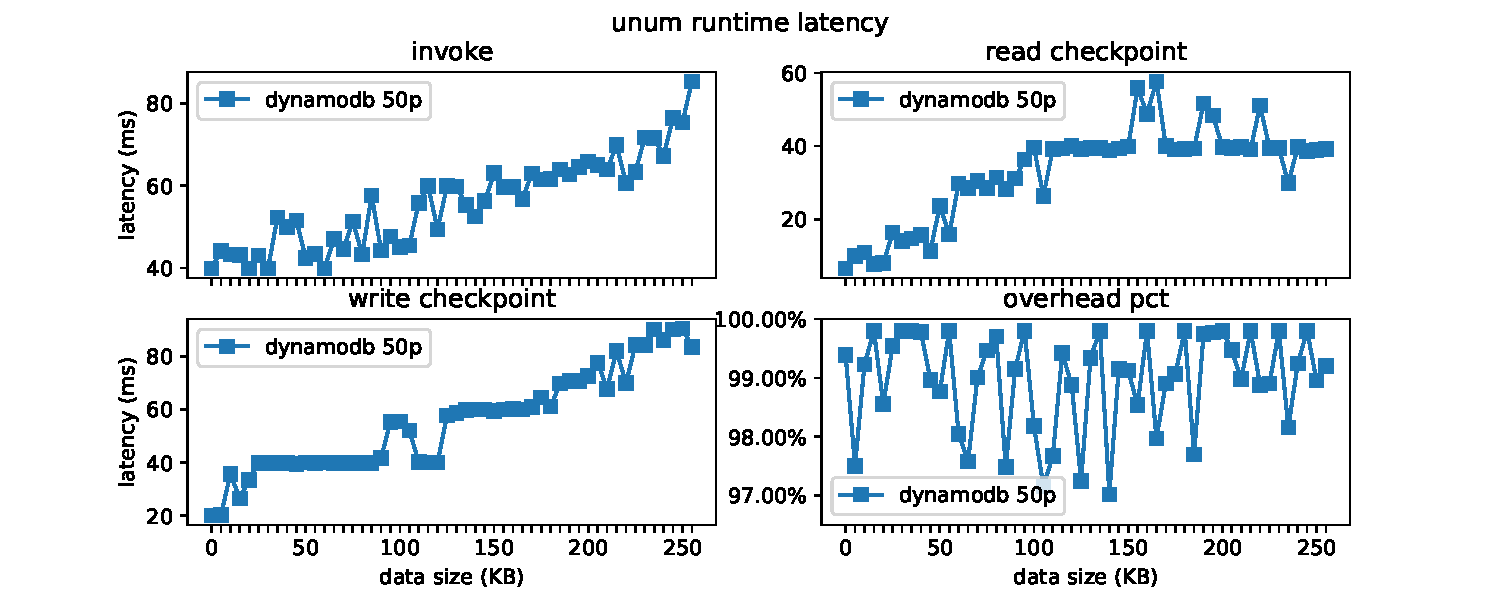
\includegraphics[width=\columnwidth]{figures/OpLatency.pdf}
    \caption{Latency of the Lambda \texttt{invoke} API for triggering a single
    function, the DynamoDB \texttt{GetItem} API for reading a checkpoint and
    the DynamoDB \texttt{PutItem} API for writing a checkpoint}
    \label{fig:oplatency}
\end{figure}

\begin{figure}[t!]
    \centering
    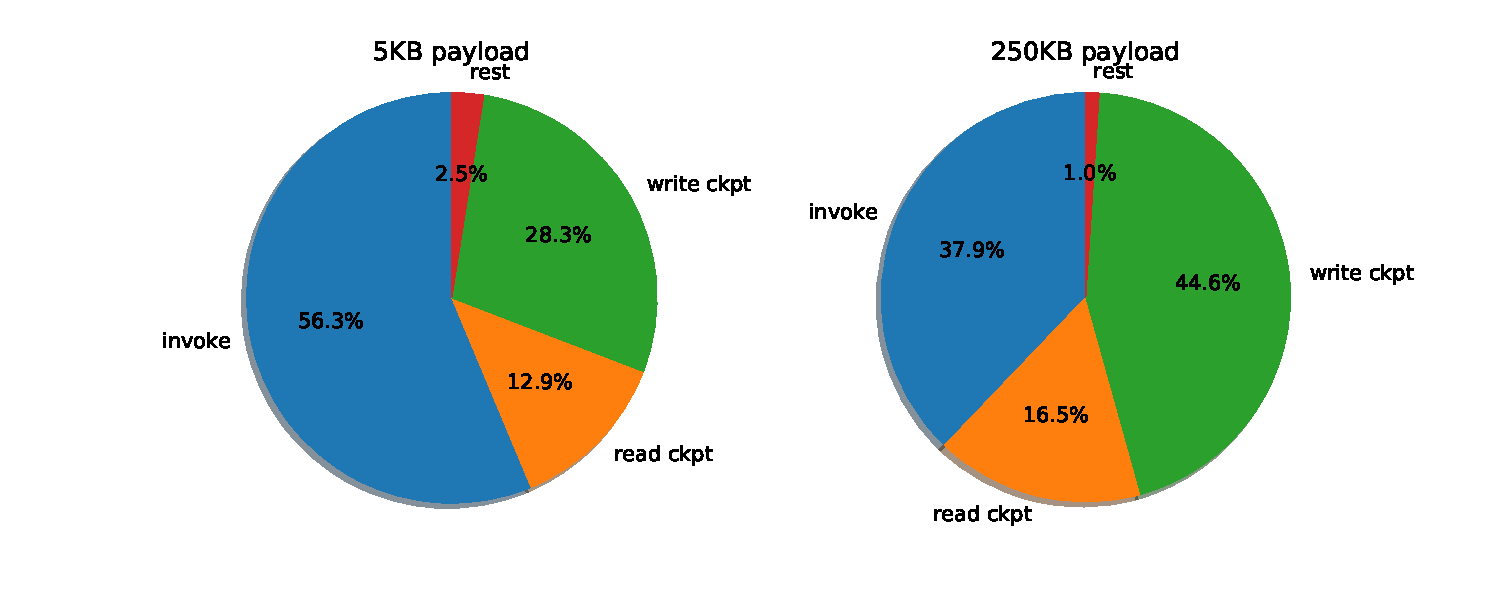
\includegraphics[width=\columnwidth]{figures/OpLatency-pct.pdf}
    \caption{Latency breakdown of the \name{} runtime. The majority of the
    latency comes from API calls to underlying services: the Lambda
    \texttt{invoke}, data store read and write.}
    \label{fig:oplatency-pct}
\end{figure}


% \paragraph{How much additional latency does unum incur? How much does that
% translate to costs?}

\subsubsection{Single transition performance}

A fundamental operation of any serverless workflow system is the transition
between a function's completion and the next function's start. The latency
of transitions bounds the end-to-end performance of workflows. In \name{},
this transition involves (1). writing a checkpoint, (2). invoking the
continuation, and (3). reading a checkpoint. That is two storage accesses and
at least one Lambda \texttt{invoke} call.

Therefore, we start our evaluation by measuring the latency of a single
transition and further breaking it down into the latencies of the Lambda
\texttt{invoke} and data store read and write API calls.

The microbenchmark we use is a chain of two functions (\texttt{F->G}) that
simply return their input without performing any computations. Invoking the
continuation involves a single call to the Lambda \texttt{invoke} API.

Because the latency of storage accesses and the Lambda \texttt{invoke} APIs
depend on how much data is written to the checkpoint and then sent to the next
function as the invocation payload, we measure across data sizes ranging
between 0-255KB in 5KB increments\footnote{Lambda limits payload size to 256KB
for async invocations.}.

As a baseline, we also measure the same latency of a state transition in Step
Functions. However, Step Functions does not generate fine-grained enough logs
for us to measure the exact apple-to-apple comparison. The results we show
measure between a \texttt{LambdaFunctionSucceeded} event and the next
\texttt{LambdaFunctionStarted} event. This is likely an underestimate because
it may not include the latency of persisting function outputs. In fact, based
on end-to-end performance of chaining (Figure~\ref{fig:chainmicrolatency}), it
is almost certain that we are not measuring all of the latency in a state
transition.

Figure~\ref{fig:totallatency} shows the total latency of a transition. \name{}
incurs 73-217ms of latency, depending on the data size. A likely underestimate
of Step Functions latency notwithstanding, \name{} is 1.09-3.54x slower than
Step Functions on a single transition.

Figure~\ref{fig:oplatency} shows the latency of the Lambda \texttt{invoke}
API, the DynamoDB \texttt{GetItem} call to read a checkpoint and the DynamoDB
\texttt{PutItem} call to write a checkpoint. Overall, all three operations
slows down as data size increases.

Figure~\ref{fig:oplatency-pct} shows the latency breakdown for 0KB data size
and 255KB data size. Over 97.5\% of the latency comes from APIs call to Lambda
and data stores. \name{} runtime code only incurs less than 2.5\% of the total
overhead. This means the bulk of \name{}'s performance will automatically
improve with the underlying platform (e.g., a faster Lambda or data store)
without any modification to \name{} itself.

\begin{figure}[t!]
    \centering
    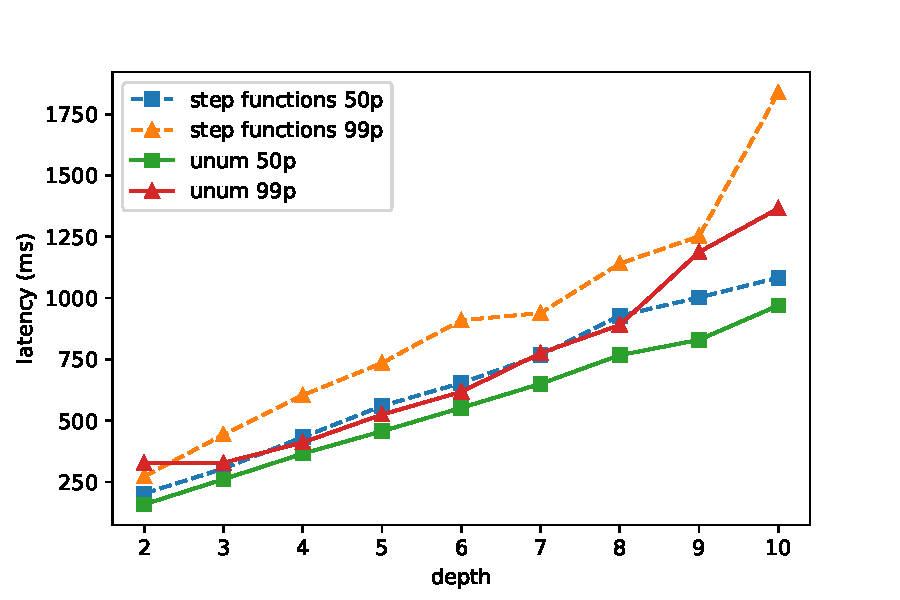
\includegraphics[width=\columnwidth]{figures/ChainMicroLatency.pdf}
    \caption{End-to-end latency of chaining N functions. Lower is
    better. Each function simply returns the input data without performing any
    computation. Results in the figure are for 1KB of input data.}
    \label{fig:chainmicrolatency}
\end{figure}

\begin{figure}[t!]
    \centering
    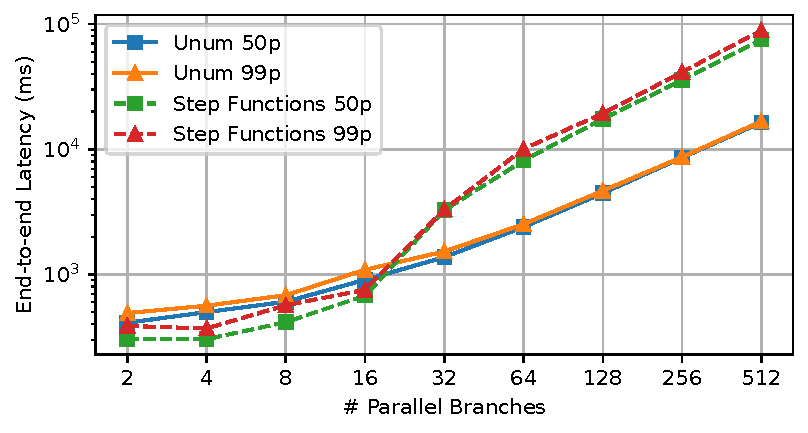
\includegraphics[width=\columnwidth]{figures/MapMicroLatency.pdf}
    \caption{End-to-end latency (logscale) of parallel fan-out and fan-in}
    \label{fig:mapmicrolatency}
\end{figure}

\subsubsection{Chaining performance}

In this section, we discuss how \name{} performs on a basic orchestration
pattern: chaining. Similarly, we use a function that simply returns its input
without any computations in this microbenchmark to minimize the runtime of
user code so that the end-to-end latency maximally reflects the performance of
the workflow system. The workflow consists of a sequential chain of the
function. We experiment with chains of varying length between 2 and 10.

Figure~\ref{fig:chainmicrolatency} shows the end-to-end latency of Step
Functions and \name{} with DynamoDB for input data size of 1KB. We also run
the same microbenchmark with 5KB and 50KB input size and the results are
similar. Overall, \name{} is around 11-28\% faster in chaining than Step
Functions.

\subsubsection{Fan-out and fan-in performance}

Next, we evaluate another critical orchestration primitive: fan-out and
fan-in. Quickly creating parallel instances is an important operation for
serverless because many applications migrate to serverless for its faster
scalability.

Step Functions has two state types, \texttt{Map} and \texttt{Parallel}, for creating
parallel branches. \name{} supports both. This microbenchmark uses the
\texttt{Map} state because it allows easy control on the number of parallel
branches.

Similarly, we use a function that simply returns its input without any
computations in this microbenchmark to minimize the runtime of user code so
that the end-to-end latency maximally reflects the performance of the workflow
system.

Figure~\ref{fig:mapmicrolatency} shows the end-to-end latency (logscale) of
fan-out and fan-in at varying levels of parallelism. At lower level of
parallelism (2-16 parallel branches), \name{} is around 100-200ms slower than
Step Functions. \name{} starts to outperform Step Functions at even moderate parallelism level of 32
parallel branches (2.37x) and up to 4.58x at 512 parallel branches.

As we do not have direct access to Step Functions's backend, it is difficult to
understand why Step Functions's performance becomes worse at higher parallelism. One
possible cause of higher latency is throttlng of concurrent branch creations.
Step Functions documentation states that it might pause creating branches when the
fan-out size exceeds 40~\cite{aws-step-functions-map-state}.

Our result is not arguing that orchestrator-based workflow systems
fundamentally scales worse than \name{}. Although Step Functions does not
elaborate on the reason for throttling, there is little reason to believe that
the maximum allowable concurrency must be capped around 40 for parallel
workloads.

However, this result does demonstrate an important downside of relying on
supplemental services to support serverless workflows. Any services added must
also perform well compared with the highly scalable FaaS engine, otherwise
application developers have to work with the restrictions that the services
impose. \name{} avoids the difficulty of building and maintaining hosted
orchestrators and directly leverages the scalability of Lambda to achieve
better parallel performance.

\subsubsection{Cost comparison}

\begin{figure}[t!]
    \centering
    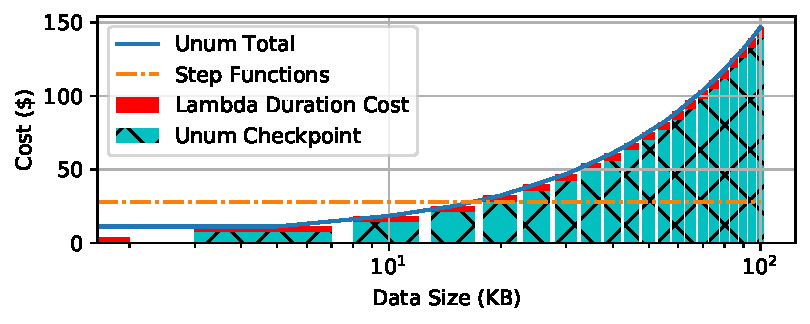
\includegraphics[width=\columnwidth]{figures/TotalCost.pdf}
    \caption{Total costs comparison of 1 million state transitions between
    Step Functions and \name{}. Computation assumes Lambda size of 3GB.}
    \label{fig:total-costs-single}
\end{figure}

\begin{figure}[t!]
    \centering
    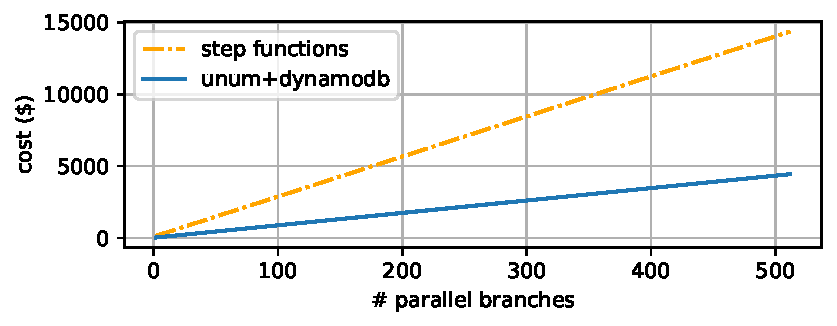
\includegraphics[width=\columnwidth]{figures/TotalMapCost.pdf}
    \caption{Total costs comparison of fan-out and fan-in between Step
    Functions and \name{}. Computation assumes Lambda size of 3GB and 1KB data
    size for function outputs and checkpoints.}
    \label{fig:total-costs-map}
\end{figure}



In this section, we break down the cost of running workflows with \name{} and
compare with that of Step Functions. We discuss the costs for a single transition,
chaining and fan-out.

Costs numbers are calculated based on AWS pricing for \texttt{us-west-1}
region. We do not "measure" the cost of running workflows because AWS does not
provide real-time billing data. We scale costs numbers by 1 million to ease
reading.

Step Functions charges based on the number of state
transitions~\cite{aws-step-functions-pricing}. Each state transition is charged
a fixed rate of \$27.9 $ \times 10^{-6}$.

There are two parts to \name{}'s costs: (1). additional Lambda duration
billing for running the \name{} runtime, and (2). data store reads and writes.

We do not count the storage costs in the intermediary data store because after
a workflow execution, checkpoints can be immediately deleted or moved to
cheaper storage by the user.

Figure~\ref{fig:total-costs-single} shows the total cost of transitions for
function data size varying between 0-255KB. The computation assumes Lambda
memory size of 3GB. We can see that the additional Lambda duration costs from
running \name{} runtime is a small fraction when compared with the costs of
DynamoDB writes. In fact, even at 255KB, the additional Lambda
duration costs is only abour \$10. If using the smallest 128MB lambdas, the
costs diminishes to merely \$0.46.

DynamoDB writes dominates the costs in \name{} because the on-demand mode
charges only not on the number of writes but also on the amount of data
written. For 1KB of data, DynamoDB charges $1.3942 \times 10^{-6}$ for a write
and $0.279 \times 10^{-6}$ for a read. Because checkpoint reads do not return
any data when there are no faults, the cost of checkpoint reads does not
increase with the data size and stays merely \$0.279 for the computation in
Figure~\ref{fig:total-costs-single}.

Even though the simulation in Figure~\ref{fig:total-costs-single} shows the
costs of \name{} outpacing that of Step Functions at larger data sizes, our
macrobenchmark results demonstrate that functions in real-world serverless
workflows do not output large amount of data. In fact, workflows tend to use
their own storage and manage application data manually. Checkpoints in the
\name{} intermediary data store are normally under 1KB.

Figure~\ref{fig:total-costs-map} shows the total costs of fan-out and fan-in
when function checkpoints are under 1KB. In addition to the costs discussed
for a single transition, the entry function performing the fan-out incurs
higher Lambda duration costs for invoking each fan-out function. The fan-in
function at the end also causes extra costs because it reads the checkpoints
of all fan-out branches. However, the total costs of this microbenchmark is
more than 3.2x lower with \name{} than Step Functions.

% \begin{itemize}

%     \item S3 charges \$5.5 per 1M PUT requests (for checkpoint write) and \$0.44
%     per 1M GET requests (for checkpoint read).

%     \item DynamoDB on-demand capcity mode charges reads and writes based on
%     the data size. 1M requests for writing 1KB data costs \$1.3942 and 1M
%     requests for reading 1KB data costs \$0.279. Note that in the case of
%     DynamoDB, if no faults happen during execution, the checkpoint read will
%     return "item not found", which costs the same as returning 1KB of data.

%     \item For 1M state transitions, \name{}'s costs for S3:

%     \[  r(d)\times0.05 + 5.94 \]

%     and for DynamoDB:

%     \[  r(d)\times0.05 + d\times1.3942 +0.279\],

%     where $r$ is the total additional runtime of \name{}, $d$ is the data
%     size.

% \end{itemize}




\subsection{Macrobenchmarks}

% \begin{table}[]
% \begin{tabular}{llllll}
% \hline
%                      &                        & \multicolumn{2}{l}{\textbf{unum}}                                                                                                   & \multicolumn{2}{l}{\textbf{Step Functions}}                                                                     \\
% \textbf{Application} & Pattern                & \textit{e2e latency} & \textit{cost (per 1M exec.)}                                                                                 & \textit{e2e latency} & \textit{cost (per 1M exec.)}                                                             \\ \hline
% IoT Pipeline         & chain                  & 120.9ms              & $0.2*2+(73+28)*$0.0021+2*\$1.3942                                                                            & 226.52               & $0.2*2+ 4*$27.9                                                                          \\
% Text Processing      & fan-out, fan-in        & 562.69ms             & $0.2*6+ (105+149+70+68+144+100)*$0.0021 + 6*$1.3942+2*2*$0.279                                               & 552.46ms             & $0.2*5+7*$27.9                                                                           \\
% Wordcount            & chain, fan-out, fan-in & 410s                 & $0.2*(1+262+1+250+1) + (277+6264*262 + 348 + 667*250 +68)*$0.0021 +(1+262+1+250+1)*$1.3942 + 262*2*$0.279+ 250*2* $0.279    & 898s                 & $0.2*(1+262+1+250+1) + (5913*262 + 154 + 633*250 +5)*$0.0021 +(1+262+1+1+250+1+1)*\$27.9 \\
% ExCamera             & chain, fan-out, fold   & 84s                  & $0.2*(1+16+15+15+14) + (6500+1500+350+4500+5000)*$0.0021+ (1+16+15+15+14)*$1.3942 + 15*2*$0.279+14*2*\$0.279 & 98s                  & $0.2*(16+16+1+16+15)+(6300+1400+2+5500+5300)*$0.0021+(1+16+16+1+1+16+1+1)*\$27.9      \\ \hline
% \end{tabular}
% \end{table}

\begin{table*}[t]
\centering
\begin{tabular}{ll|cc|cc}
\hline
                     &                        & \multicolumn{2}{c}{\textbf{\name{}}}            & \multicolumn{2}{c}{\textbf{Step Functions}}       \\
\textbf{Application} & \textbf{Pattern}       & \textit{e2e latency} & \textit{cost (per 1 mil. exec.)}   & \textit{e2e latency} & \textit{cost (per 1 mil. exec.)}            \\ \hline
IoT Pipeline         & chain                  & 120.9ms              & \$3.4005      & 226.52       & \$111.6    \\
Text Processing      & fan-out, fan-in        & 562.69ms             & \$12.0168      & 552.46ms             & \$196.3                                                                           \\
Wordcount            & chain, fan-out, fan-in & 410s                 & \$4904.79   & 898s                 & \$18113 \\
ExCamera             & chain, fan-out, fold   & 84s                  & \$150.91 & 98s                  & \$1530      \\ \hline
\end{tabular}
\caption{Latency and costs comparison between \name{} and Step Functions for the macrobenchmark applications}
\label{table:macro}
\end{table*}

We further evaluate \name{}'s performance, costs and expressiveness with 4
real-world applications. 

\paragraph{IoT Pipeline} Adapted from a humidity control application in the
AWS serverless repository~\cite{iot-pipeline}. The workflow consists of a
chain of two functions that processes climate control data and change the HVAC
setting.

\paragraph{Text Processing} Adapted from the social network application in
DeathStarBench~\cite{deathstar}. The workflow consists of 5 functions that
create a social network post by processing user mentions, shortening URLs and
eventually saving the post in a DynamoDB table.

\paragraph{Wordcount} MapReduce word count~\cite{mapreduce} ran with 250
parallel mappers and reducers.

\paragraph{ExCamera} The ExCamera video encoder~\cite{excamera, gg-atc}. We
use the same workload and setup as the experiment in gg~\cite{gg-atc}: the same
input video of the first 888 chunks of sintel 4K, 3GB lambdas and 16 chunks
per batch.

Table~\ref{table:macro} lists the median end-to-end latency and computed costs
per 1 million executions. Both latency and costs numbers are based on DynamoDB
as the intermediary data store. \name{} is slower than Step Functions for Text
Processing where the workflow fans out to 2 parallel branches. However,
\name{} is faster in the other applications that consists of chaining and
fan-outs at much higher level of parallelism.

Furthermore, \name{} is consistently cheaper than Step Functions for all
workloads with 3.7x to 32.8x costs savings. Most applications manually manage
application data with their own storage and function checkpoints are smaller
than 1KB for all 4 workflows.

\subsubsection{ExCamera}

\begin{itemize}

    \item \name{} is able to express and execute parallel pipelines while Step
    Functions has to serialize the decode and re-encode stages.

    \item Step Functions does not have a way to express fold, so the last
    rebase stage has to be written as a single recursive function. \name{}
    supports fold. The recursion logic is lifted to the \name{} IR and the
    rebase function is written similarly to ExCamera.

    \item \name{} is 7.1\% faster than gg's implementation of ExCamera and
    \%10.5 slower than the original ExCamera. Similar to gg, \name{} also do
    not pre-load the input data from S3. Different from gg, \name{} does not
    use a long-running coordinator on EC2 to manage communications and
    invocations.

\end{itemize}

\subsubsection{Questions}

\begin{enumerate}

    \item How do we evaluate and present execution guarantee? Anything to show
     to convince our reader that it's correct?

    \item How do we evaluate other benefits that stem from a simpler design
     (the fact that unum gets rid of the needs for a separate orchestrator
     service), such as resource management, required staffing and other
     hosting costs? Further on the resource utilization point, do we want to
     say that dollar costs of running applications is a reasonable enough
     proxy to resource consumption and therefore lower price = less resource
     consumption = better resource utilization?

    \item Should we run experiments with S3 and present those numbers?

    \item How to discuss the expressiveness advantage? Specifically,

        Step Functions has no way to express a for loop or fold.

        Step Functions has no way to express pipeline parallelism.

        Step Functions fan-in needs to make sure the aggregate data doesn't exceed a
        limit, unum automatically passes data in using pointers to the intermediary
        data store.

\end{enumerate}

